\documentclass{article}
\usepackage{graphicx}

%% http://www.ctan.org/tex-archive/help/Catalogue/entries/igo.html
\usepackage{igo}
\gobansize{9}

\usepackage[empty,cm]{fullpage}
\begin{document}

%% The first page includes a 9x9 board.
\hbox{}
\vfill

\begin{center}
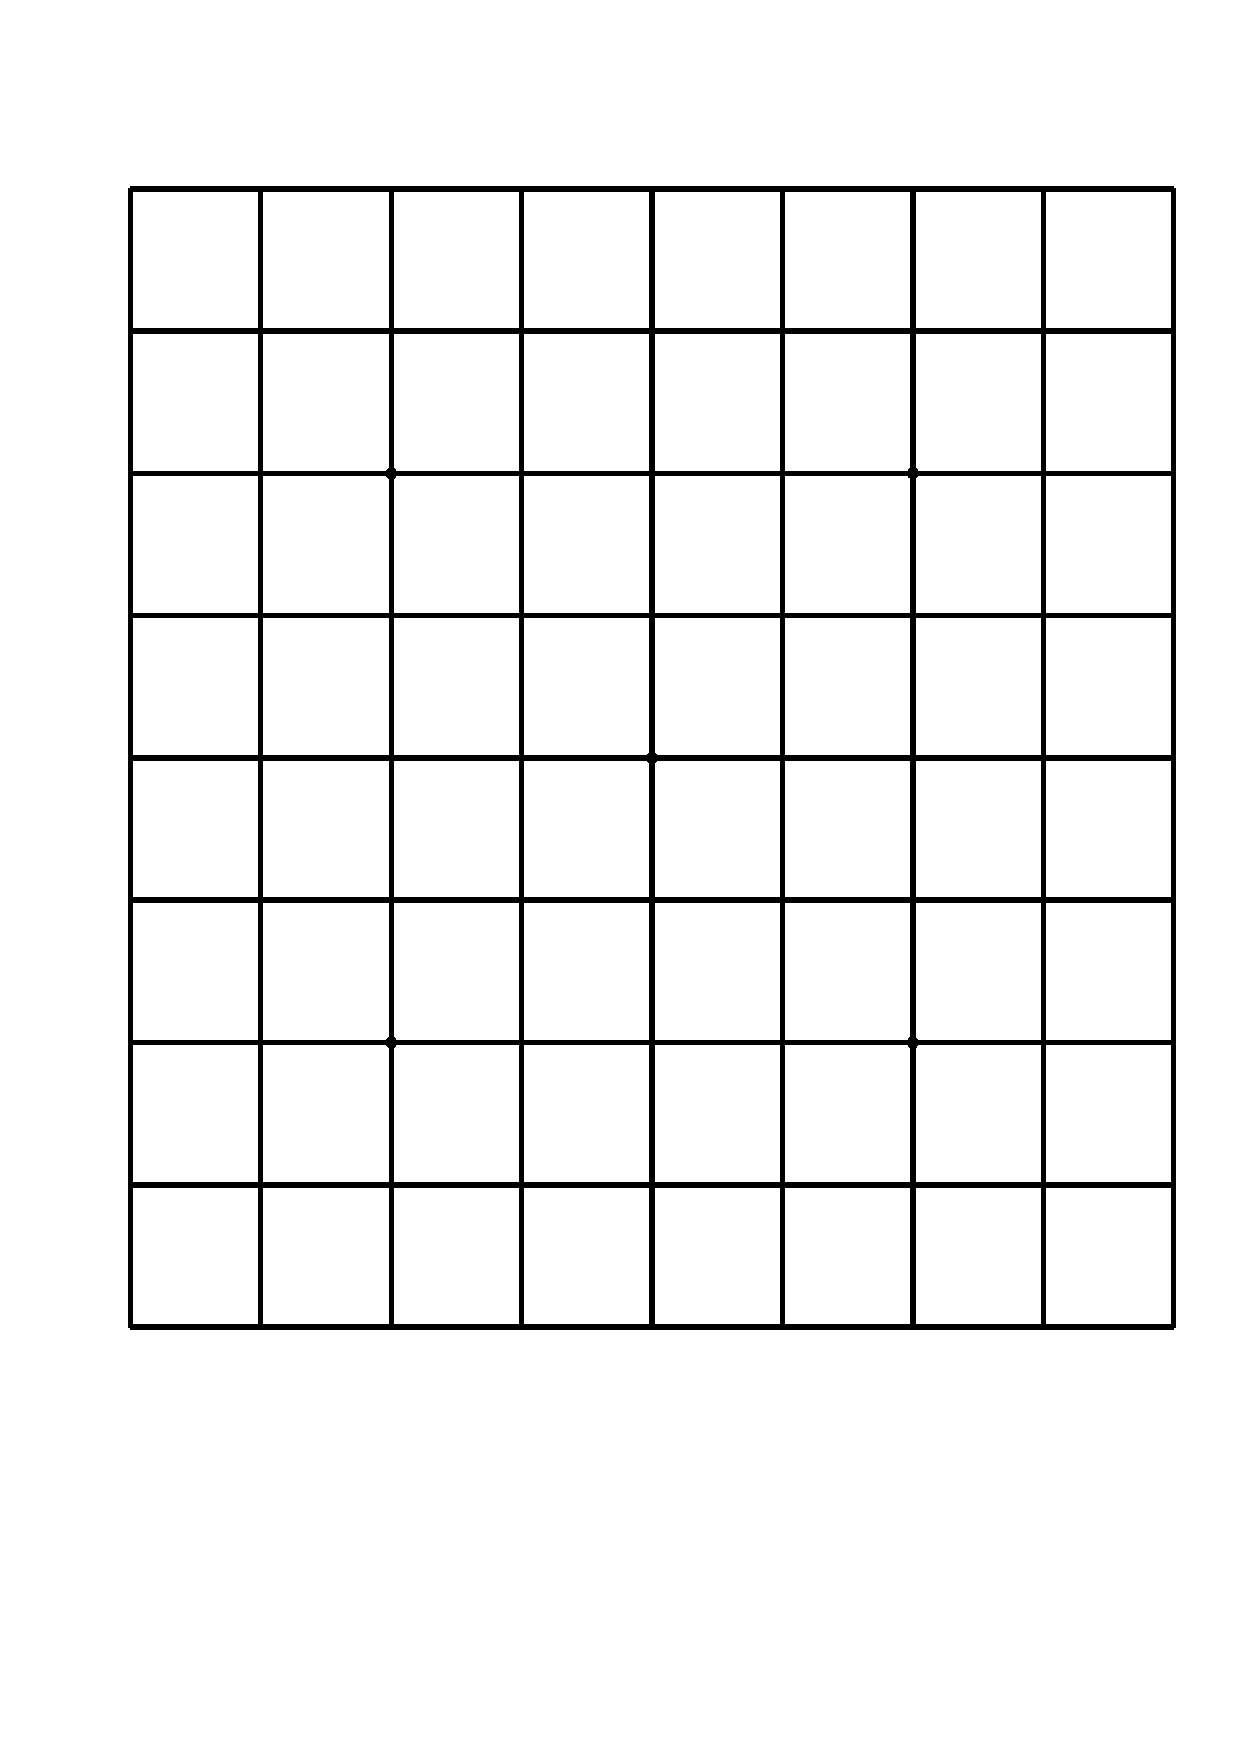
\includegraphics{gb9.epsi}
\end{center}

\vfill

\newpage

%% The next page includes a small description of the capturing rules,
%% a few puzzles, and references for more information.
\section*{Introduction}
Go is a board game between black and white.  Like Chess, black and
white take turns, and black goes first.  Unlike Chess, the board
starts empty, and the goal is not necesarily to capture the opponent's
pieces, but to take majority control of the board.

That being said, control of the board is intimately related to
capture, so let's talk about the capturing rule.




\section*{Puzzles}

%% Game taken from http://www.societies.cam.ac.uk/cugos/go/rules_06.html
\section*{A 9x9 Game}
To help give an impression of the game, here's an example of a full game.
%
\begin{center}
\shortstack{
\black[1]{d7,f4,c4,f7,f6,g6,f5,g5,g7,f8}
\showfullgoban\\Moves 1--10.}
\hspace{1in}%
\shortstack{
\cleargobansymbols
\black[11]{e7,g8,e4,f3,e3,e2,d2,f2,c3,c9}
\showfullgoban\\Moves 11--20.}
\hspace{1in}%
\shortstack{\cleargoban
\cleargobansymbols
\black[21]{}
\showfullgoban\\Moves 21--30.}
\end{center}
%
In this game, black and white are jostling and pushing against each
other.  Black has emphasized the left side of the board, white the
right side.



\end{document}
